\chapter{数列}
\section{差分与求和}
如果有一个数列$\{a_n\}$,可以定义它的差分$\Delta a_n=a_n-a_{n-1}$,求和$\Sigma a_n=a_1+a_2+\dots+a_n$。(它们是一对逆运算,$\Delta \Sigma a_n=a_n$。有些地方会定义$\Delta a_n=a_{n+1}-a_{n}$,这样不太方便。)

比如$\Delta n^2=2 n-1$,$\Sigma n^2=\frac{1}{6}n(n+1)(2 n+1)$。像$n^4+2 n^3+3 n$这样的多项式可以一项一项差分或者求和,也就是说差分与求和都是线性算符。

差分算符$\Delta$与求和算符$\Sigma$跟求导算符$\ddx$与积分算符$\int \opd x$很像。这个积分算符表示的是不定积分,所以这个求和算符其实是“不定”求和。比如“定”求和$\sum_{n=38}^{62} n^2$用这个求和算符就要表示成$\Sigma n^2|_{n=62}-\Sigma n^2|_{n=37}$。数列差分与求和的时候,下标加减$1$的情况比微积分还要麻烦。

上面的求和是从$1$开始的,其实不一定要从$1$开始,相当于“不定”求和出来的常数换一下,对计算“定”求和没有影响。

如果要与微积分更像一点,可以把差分与求和写成$\frac{\Delta}{\Delta n}$与$\Sigma \Delta n$。但是一般情况下$\Delta n=1$,所以可以省略,否则要进行换元。比如$1+3+5+\dots$可以表示成$\Sigma n \Delta n$,其中$\Delta n=2$。令$n=2 m-1$,这样$m=\frac{n+1}{2}$,$\Delta m=\frac{1}{2} \Delta n=1$,而且$m=1$时$n=1$,这样“不定”求和的起点是一致的。换元之后就得到$\Sigma n \Delta n=\Sigma (2 m-1) \Delta m=2 \cdot \frac{1}{2} m(m+1) -m=m^2=\frac{(n+1)^2}{4}$。
\section{用递推求$\Sigma n^p$}
我们都知道$\Sigma n=\frac{1}{2}n(n+1)$,现在来推导$\Sigma n^2$。我们不直接考虑$\Sigma n^2$,而是先考虑$\Sigma n^3$:
\begin{align*}
\Sigma n^3+(n+1)^3&=\sum_{k=1}^{n+1} k^3 \\
&=\sum_{k=0}^n (k+1)^3 \\
&=\sum_{k=0}^n (k^3+3 k^2+3 k+1) \\
&=\Sigma n^3+3 \Sigma n^2+\frac{3}{2}n(n+1)+(n+1)
\internote{(两边的$\Sigma n^3$可以消掉,$\sum_{k=0}^n 1=n+1$)}
3 \Sigma n^2&=(n+1)^3-\frac{3}{2}n(n+1)-n-1 \\
\Sigma n^2&=\frac{n^3}{3}+\frac{n^2}{6}+\frac{n}{2} \\
&=\frac{1}{6}n(n+1)(2 n+1)
\end{align*}

用类似的方法,对任何正整数$p$,如果知道$\Sigma n,\Sigma n^2,\dots,\Sigma n^{p-1}$,就能求出$\Sigma n^p$。这是一种递推的方法,而且第二步打开$(k+1)^{p+1}$需要计算组合数,当$p$增大的时候需要很大的计算量。

【练习】证明$\Sigma n^3=\frac{1}{4}n^2 (n+1)^2$。

并没有简单(复杂度与$p$无关)的公式可以计算$\Sigma n^p$。如果$p$是实数甚至复数,问题就更复杂了。传说中的\emph{黎曼zeta函数}就是$\zeta(z)=\sum_{k=0}^{\infty} k^z$,在现代数学中十分重要。一个简单的结论是:$z$是实数且$z<-1$时,$\zeta(z)$收敛;$z \ge -1$时,$\zeta(z)$发散。
\section{降幂;离散微积分}
再来讲另一种计算$\Sigma n^p$的方法。先定义一个“降幂”运算:$\dspw{n}{p}=n \cdot (n-1) \cdot (n-2) \cdot \dots \cdot (n-p+1)$,其中$n$是实数,$p$是正整数。比如$\dspw{n}{4}=n(n-1)(n-2)(n-3)$。(也可以定义“升幂”,但是不常用)

然后我们发现了喜闻乐见的事情:$\Delta \dspw{n}{p}=p \dspw{(n-1)}{p-1}$,$\Sigma \dspw{n}{p}=\frac{1}{p+1} \dspw{(n+1)}{p+1}$。这两个公式和微积分里的差不多,但是要注意$n$的加减。

举个栗子,$\Delta \dspw{n}{3}=n(n-1)(n-2)-(n-1)(n-2)(n-3)=3(n-1)(n-2)=3 \dspw{(n-1)}{2}$。直接计算降幂的求和可以用一加一减的技巧,比如
\begin{align*}
\Sigma \dspw{n}{2}&=2 \cdot 1+3 \cdot 2 +\dots+ n(n-1) \\
&=\frac{1}{3}(3 \cdot 2 \cdot 1-2 \cdot 1 \cdot 0+4 \cdot 3 \cdot 2-3 \cdot 2 \cdot 1+\dots+(n+1)n(n-1)-n(n-1)(n-2)) \\
&=\frac{1}{3}(n+1)n(n-1) \\
&=\frac{1}{3} \dspw{(n+1)}{3}
\end{align*}

因为求和的下限是$2$,这个结果在$n \ge 2$时成立,$n=1$时要另外讨论。

组合数中经常出现$n \cdot (n-1) \cdot (n-2) \dots$这样的式子,如果你熟悉组合数的公式,可以推导出这两个公式。

降幂的差分与求和容易计算,但是把普通的幂转换成降幂是不容易的,可以用类似于整式除法的方法,比如$n^2=\dspw{n}{2}+\dspw{n}{1}$,$n^3=\dspw{n}{3}+3 \dspw{n}{2}+\dspw{n}{1}$,$n^4=\dspw{n}{4}+6 \dspw{n}{3}+7 \dspw{n}{2}+\dspw{n}{1}$。

有兴趣的同学可以把$\Sigma n^3,\Sigma n^4$推导一遍,还可以检验一下这种方法的复杂度和递推是一样的。

到现在为止$p$是正整数,如果$p$是$0$或者负整数怎么办呢?因为$\frac{\dspw{n}{p}}{\dspw{n}{p-1}}=n-p+1$,令$p=1$,得到$\frac{\dspw{n}{1}}{\dspw{n}{0}}=n$,所以$\dspw{n}{0}=1$。类似地可以定义$\dspw{n}{-1}=\frac{1}{n+1},\dspw{n}{-2}=\frac{1}{(n+1)(n+2)},\dots$

上面的差分与求和公式仍然成立,现在直接计算降幂的求和可以通过裂项,比如
\begin{align*}
\Sigma \dspw{n}{-3}&=\frac{1}{1 \cdot 2 \cdot 3}+\frac{1}{2 \cdot 3 \cdot 4}+\dots+\frac{1}{(n+1)(n+2)(n+3)} \\
&=\frac{1}{2}(\frac{1}{1 \cdot 2}-\frac{1}{2 \cdot 3}+\frac{1}{2 \cdot 3}-\frac{1}{3 \cdot 4}+\cdots+\frac{1}{(n+1)(n+2)}-\frac{1}{(n+2)(n+3)}) \\
&=\frac{1}{2}(\frac{1}{2}-\frac{1}{(n+2)(n+3)})
\end{align*}

这里求和的下限是$0$。因为是“不定”求和,可以去掉括号中的$\frac{1}{2}$,得到$\Sigma \dspw{n}{-3}=\frac{1}{-2} \cdot \frac{1}{(n+2)(n+3)}=\frac{1}{-2}\dspw{(n+1)}{-2}$。在计算“定”求和时仍然要注意边界,比如$\frac{1}{1 \cdot 2 \cdot 3}+\frac{1}{2 \cdot 3 \cdot 4}+\dots+\frac{1}{(n-2)(n-1)n}=\Sigma \dspw{k}{-3}|_{k=n-3}-\Sigma \dspw{k}{-3}|_{k=-1}=\frac{1}{-2}(\dspw{0}{-2}-\dspw{(n-2)}{-2})=\frac{1}{-2}(\frac{1}{1 \cdot 2}-\frac{1}{(n-1)n})$。

但是!$p=0$时,$\Delta \dspw{n}{p}=\Delta 1=0$。$p=-1$时,$\Sigma \dspw{n}{p}=\frac{1}{1}+\frac{1}{2}+\frac{1}{3}+\dots$,没有简单的表示方法,我们把它叫做调和级数$H_n$。它们是特殊情况。

上面讲的是幂函数的差分与求和,而对于指数函数,$\Delta q^n=(q-1) q^{n-1}$,$\Sigma q^n=\frac{1}{q-1} q^{n+1}$。

当$n$很大时,$\dspw{n}{p}$的增长速度与$n^p$差不多,也就是说它们的相对误差趋于$0$。(当然绝对误差会越来越大)而$H_n$的增长速度与$\ln n$差不多,对应$\int \frac{1}{x} \opd x=\ln x$。

如果令$n \rightarrow \infty$,$\Delta k \rightarrow 0$,而$n \Delta k$为恒定值$a$,那么求和$\sum_{k=0}^n f(k) \Delta k$将会趋于积分$\int_{x=0}^a f(x) \opd x$,这就是高考当中微元法的理论基础。(黎曼积分之类的严格定义以后再讲)
\section{阿贝尔变换;分部求和}
数列的乘积的差分也有与微积分中对应的公式,也就是阿贝尔变换:
\begin{align*}
\Delta(a_n b_n)&=a_n b_n-a_{n-1} b_{n-1} \\
&=a_n b_n+a_n b_{n-1}-a_n b_{n-1}-a_{n-1} b_{n-1} \\
&=a_n(b_n-b_{n-1})+b_{n-1}(a_n-a_{n-1}) \\
&=a_n \Delta b_n+b_{n-1} \Delta a_n
\end{align*}

也可以写成$a_{n-1} \Delta b_n+b_n \Delta a_n$。这里也用了一加一减的技巧。与分部积分对应的则是
\begin{equation*}
\Sigma a_n \Delta b_n=a_n b_n-\Sigma b_{n-1} \Delta a_n
\end{equation*}

举个栗子:
\begin{align*}
\Sigma n q^n \Delta n&=\frac{1}{q-1} \Sigma n \Delta q^{n+1} \\
&=\frac{1}{q-1}(n q^{n+1}-\Sigma q^n \Delta n)
\internote{(注意后面的求和不是$\Sigma q^{n+1}$)}
&=\frac{1}{q-1}(n q^{n+1}-\frac{1}{q-1} q^{n+1}) \\
&=\frac{q}{(q-1)^2}((q-1)n-1)q^n
\end{align*}

高考范围内应该会用作差法算这个求和,这样分部求和的计算量其实差不了多少,方便之处在于跟微积分中计算$\int x \rme^x \opd x$的套路一样。而且先算“不定”求和,最后再考虑上下限,可能比每一步都考虑上下限方便一点。

再举个复杂一点的例子:
\begin{align*}
\Sigma n^2 3^n \Delta n&=\frac{1}{2} \Sigma n^2 \Delta 3^{n+1} \\
&=\frac{1}{2}(n^2 3^{n+1}-\Sigma 3^n \Delta n^2) \\
&=\frac{1}{2}(n^2 3^{n+1}-\Sigma 3^n (2 n-1) \Delta n) \\
&=\frac{1}{2} n^2 3^{n+1}-n \Sigma 3^n \Delta n+\frac{1}{2} \Sigma 3^n \Delta n \\
&=\frac{1}{2} n^2 3^{n+1}-\frac{3}{4}(2 n-1) 3^n+\frac{1}{4} 3^{n+1} \\
&=\frac{3}{2}(n^2-n+1) 3^n
\end{align*}

【练习】求$\Sigma n^2 (\frac{1}{2})^n$,然后证明$\sum_{n=1}^{\infty}n^2 (\frac{1}{2})^n=6$。

遗憾的是,微积分中比值的导数和复合函数的导数,在数列中没有好看的公式与之对应。
\section{多重求和与交换顺序}
多个求和号放在一起,默认从右往左计算。如果两次求和的上下限与被求和的变量无关,那么它们的顺序是可以交换的,比如
\begin{equation*}
\sum_{i=i_\text{min}}^{i_\text{max}} \sum_{j=j_\text{min}}^{j_\text{max}} a_{i j}=\sum_{j=j_\text{min}}^{j_\text{max}} \sum_{i=i_\text{min}}^{i_\text{max}} a_{i j}
\end{equation*}

其中$i_\text{min}$和$i_\text{max}$都是常数,与$j$无关;$j_\text{min}$和$j_\text{max}$也与$i$无关。这其实就是加法交换律。

上下限与被求和变量有关的情况就比较麻烦。比如
\begin{equation*}
\sum_{i=1}^4 \sum_{j=1}^i a_{i j}=\sum_{j=1}^4 \sum_{i=j}^4 a_{i j}
\end{equation*}

从图\ref{fig-triangle-sum}中可以看出,等号左边表示一行一行加起来,右边则表示一列一列加起来。
\begin{figure}[htb]
\centering
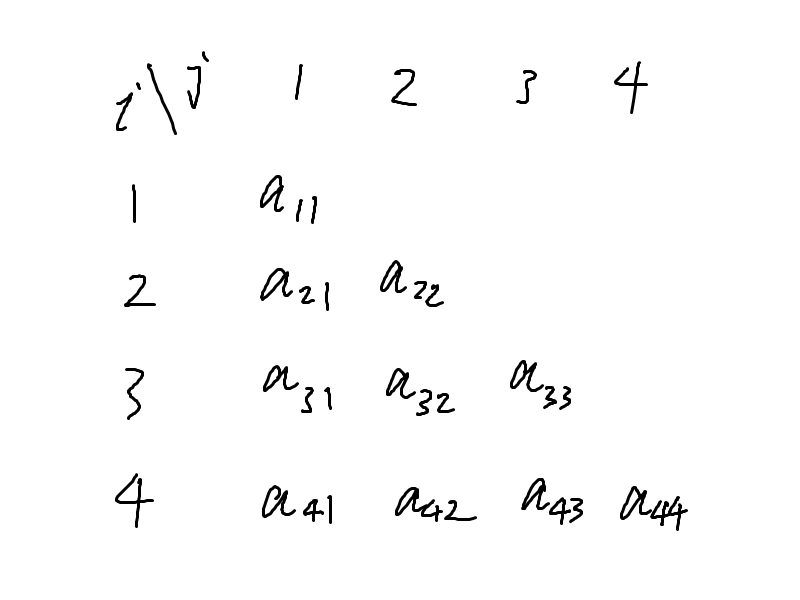
\includegraphics[scale=0.5]{fig/triangle-sum}
\caption{把三角形里面的东西求和}
\label{fig-triangle-sum}
\end{figure}

现在来对前面的调和级数再进行一次求和:
\begin{align*}
\Sigma H_{n-1}&=\sum_{i=1}^{n-1} \sum_{j=1}^i \frac{1}{j}=\sum_{j=1}^{n-1} \sum_{i=j}^{n-1} \frac{1}{j}=\sum_{j=1}^{n-1} \frac{n-j}{j} \\
&=\sum_{j=1}^{n-1} (\frac{n}{j}-1)=\sum_{j=1}^{n} (\frac{n}{j}-1)=n H_n-n
\end{align*}

($j=n$时$\frac{n}{j}-1=0$,但是把上限从$n-1$改为$n$会让结果好看一些)

所以$\Sigma H_{n-1}=n H_n-n$,它对应$\int \ln x \opd x=x \ln x-x$。$n=5$时,可以用图\ref{fig-triangle-harmonic}来表示。
\begin{figure}[htb]
\centering
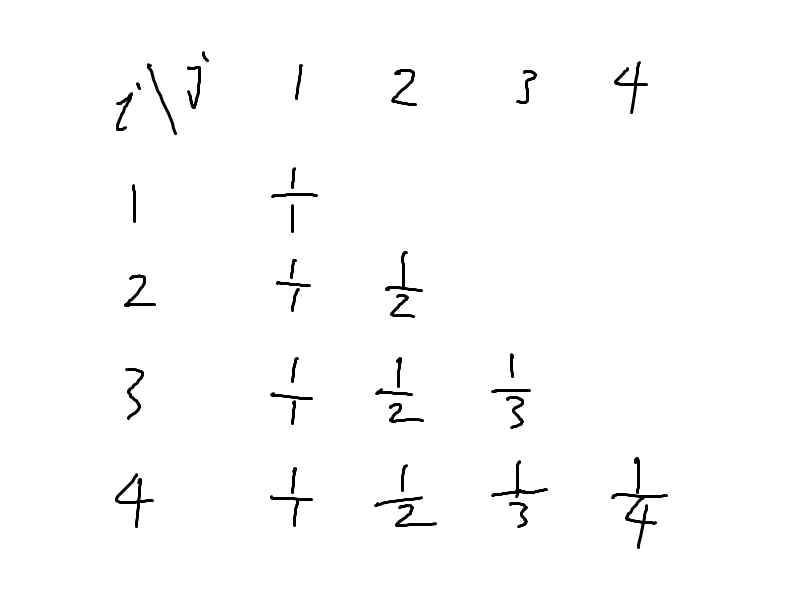
\includegraphics[scale=0.5]{fig/triangle-harmonic}
\caption{把调和级数排成三角形}
\label{fig-triangle-harmonic}
\end{figure}

(用分部求和也可以算出这个结果,我只是想给多重求和举个栗子)
\section{差分方程}
差分方程其实就是我们平常说的递推式,它与微分方程有许多相似的地方。(建议先看前面微分方程的内容)

比如解二阶线性常系数齐次差分方程(现在你应该可以猜出这一长串名字是什么意思了)
\begin{equation*}
a_{n+2}+p a_{n+1}+q a_n=0
\end{equation*}

有些地方会让我们算“特征方程”$\lambda^2+p \lambda+q=0$,为什么要这样做呢?其实我们先猜$a_n=\lambda^n$,代入方程得到$\lambda^{n+2}+p \lambda^{n+1}+q \lambda^n=0$,除以$\lambda^n$就得到这个特征方程。

解出两个根$\lambda_1$和$\lambda_2$,通解就是$a_n=A \lambda_1^n+B \lambda_2^n$,可以通过边界条件确定$A$和$B$。

如果$\lambda_1$和$\lambda_2$是复数,数列就会出现周期性。如果$\lambda_1=\lambda_2$,就要重新猜解:$a_n=(A n+B)\lambda^n$。跟前面阻尼振动的讨论一样。

(差分方程要讲的只有这么多,各种奇怪的非线性差分方程就不讲了,很多书上都有)
\section{数列在不动点附近的收敛}
高考经常会出这样的题:已知$a_{n+1}=f(a_n)$,求证$\Sigma a_n<S$,$S$可能是常数或者$n$的函数。

其中的函数$f(x)$一般有不动点$x_0$,也就是说$f(x_0)=x_0$。如果你偷偷按过计算器,会发现$a_n$收敛到$x_0$,否则这道题就没法做了。不动点可能不止一个,一般$a_n$会收敛到最近的那个。为了方便,可以移动坐标原点让$x_0=0$,也就是说$f(0)=0$。

如果$|a_n| \ll 1$,可以把$f(a_n)$作泰勒展开:$a_{n+1}=f(a_n)=k_1 a_n+k_2 a_n^2+\dots$,取最低阶近似得到$a_{n+1}=k_1 a_n$,$k_1=f'(0)$。如果$k_1<1$,$a_n$就近似是一个收敛的等比数列,然后再求和。

但是初始条件可能不满足$|a_1| \ll 1$,这时可以先算出前几项,再把剩下的近似成等比数列。只要这道题的答案是存在的,我们总可以放掉有限项,剩下的近似成等比数列。如果放掉的项数太多,超出了手算的能力,那就要考虑其他思路,比如裂项或者整体代换。

($|a_n| \ll 1$到底要多小,很难作出准确的描述。即使$a_n$很小,泰勒级数后面的无穷多项加起来也可能有比较大的影响,这里就不仔细讲了)
